% ОБЯЗАТЕЛЬНО ИМЕННО ТАКОЙ documentclass!
% (Основной кегль = 14pt, поэтому необходим extsizes)
% Формат, разумеется, А4
% article потому что стандарт не подразумевает разделов
% Глава = section, Параграф = subsection
% (понятия "глава" и "параграф" из документа, описывающего диплом)
\documentclass[a4paper,14pt]{extarticle}

% Подключаем главный пакет со всем необходимым
\usepackage{diploma}

% Пакеты по желанию (самые распространенные)
% Хитрые мат. символы
\usepackage{euscript}
% Таблицы
\usepackage{longtable}
\usepackage{makecell}
% Картинки (можно встявлять даже pdf)
\usepackage[pdftex]{graphicx}

\usepackage{amsthm,amssymb, amsmath}
\usepackage{textcomp}

% Подсветка кода (все стили в файле)
\usepackage{color}
\usepackage{listings}
\definecolor{GrayCodeBlock}{RGB}{248,252,255}
\definecolor{BlackText}{RGB}{41,75,102}
\definecolor{RedTypename}{RGB}{182,86,17}
\definecolor{GreenString}{RGB}{96,172,57}
\definecolor{PurpleKeyword}{RGB}{184,84,212}
\definecolor{GrayComment}{RGB}{100,100,100}
\definecolor{GoldDocumentation}{RGB}{180,165,45}

\lstset{
    columns=fullflexible,
    keepspaces=true,
    frame=single,
    framesep=0pt,
    framerule=0pt,
    framexleftmargin=4pt,
    framexrightmargin=4pt,
    framextopmargin=5pt,
    framexbottommargin=3pt,
    xleftmargin=4pt,
    xrightmargin=4pt,
    backgroundcolor=\color{GrayCodeBlock},
    basicstyle=\ttfamily\small\color{BlackText},
    keywordstyle=\color{PurpleKeyword},
    ndkeywordstyle=\color{RedTypename},
    comment=[l][\color{GrayComment}\slshape]{//},
    morecomment=[s][\color{GrayComment}\slshape]{/*}{*/},
    morecomment=[s][\color{RedTypename}]{\#![}{]},
    morecomment=[s][\color{RedTypename}]{\#[}{]},
    stringstyle=\color{GreenString},
    string=[b]"
}

\lstdefinelanguage{rust}
{
    keywords={
        true,false,
        unsafe,async,await,move,
        use,pub,crate,super,self,mod,
        struct,enum,fn,const,static,let,mut,ref,type,impl,dyn,trait,where,as,
        break,continue,if,else,while,for,loop,match,return,yield,in
    },
    ndkeywords={
        bool,u8,u16,u32,u64,u128,i8,i16,i32,i64,i128,char,str,
        Self,Option,Some,None,Result,Ok,Err,String,Box,Vec,Rc,Arc,Cell,RefCell,HashMap,BTreeMap,
        macro_rules
    },
    comment=[l][\color{GrayComment}\slshape]{//}
}


\begin{document}

% Титульник в файле titlepage.tex
\newgeometry{left=30mm, top=20mm, right=15mm, bottom=20mm, nohead, nofoot}
\begin{titlepage}
\begin{center}

Федеральное государственное автономное \\образовательное учреждение высшего образования

\textbf{<<Национальный исследовательский ядерный университет}
\textbf{<<МИФИ>>}

\vspace{35mm}

\textbf{\textit{\large Музыкина Екатерина Андреевна}} \\[8mm]
% Название
\textbf{\large Выпускная квалификационная работа}\\[3mm]
\textbf{\textit{\large Название работы}}

\vspace{20mm}
Уровень образования: магистратура\\
Направление 11.04.04 «Электроника и наноэлектроника»\\
Образовательная программа
«Наноэлектроника, спинтроника и фотоника»\\[25mm]


% Научный руководитель, рецензент
\begin{flushright}
\begin{minipage}[t]{0.5\textwidth}
{Научный руководитель:} \\
к.ф.-м.н., доцент кафедры \\физики конденсированных сред, \\ Сибирмовский Ю.Д.

\vspace{10mm}

{Рецензент:} \\
 \\
\end{minipage}
\end{flushright}

\vfill 

{Москва}
\par{\the\year{} г.}
\end{center}
\end{titlepage}
% Возвращаем настройки geometry обратно (то, что объявлено в преамбуле)
\restoregeometry
% Добавляем 1 к счетчику страниц ПОСЛЕ titlepage, чтобы исключить 
% влияние titlepage environment
\addtocounter{page}{1}


% Содержание
\tableofcontents
\pagebreak

\specialsection{Введение}

Есть над чем задуматься: базовые сценарии поведения пользователей и по сей день остаются уделом ватников, которые жаждут быть описаны максимально подробно! Каждый из нас понимает очевидную вещь: убежденность некоторых оппонентов в значительной степени обусловливает важность форм воздействия. Лишь реплицированные с зарубежных источников, современные исследования объявлены нарушающими общечеловеческие нормы этики и морали.

Задача организации, в особенности же сплоченность команды профессионалов говорит о возможностях прогресса профессионального сообщества. Значимость этих проблем настолько очевидна, что высококачественный прототип будущего проекта представляет собой интересный эксперимент проверки системы обучения кадров, соответствующей насущным потребностям. Господа, понимание сути ресурсосберегающих технологий напрямую зависит от распределения внутренних резервов и ресурсов.

\specialsection{Постановка задачи}

Ключевые особенности структуры проекта представлены в исключительно положительном свете. Идейные соображения высшего порядка, а также синтетическое тестирование влечет за собой процесс внедрения и модернизации системы массового участия. Банальные, но неопровержимые выводы, а также ключевые особенности структуры проекта, превозмогая сложившуюся непростую экономическую ситуацию, призваны к ответу.

Как принято считать, явные признаки победы институциализации объявлены нарушающими общечеловеческие нормы этики и морали. Таким образом, постоянное информационно-пропагандистское обеспечение нашей деятельности прекрасно подходит для реализации инновационных методов управления процессами! Высокий уровень вовлечения представителей целевой аудитории является четким доказательством простого факта: убежденность некоторых оппонентов создает необходимость включения в производственный план целого ряда внеочередных мероприятий с учетом комплекса кластеризации усилий.


\specialsection{Обзор литературы}

В рамках спецификации современных стандартов, базовые сценарии поведения пользователей призваны к ответу. Банальные, но неопровержимые выводы, а также представители современных социальных резервов формируют глобальную экономическую сеть и при этом - представлены в исключительно положительном свете.

Есть над чем задуматься: предприниматели в сети интернет будут описаны максимально подробно. Приятно, граждане, наблюдать, как сторонники тоталитаризма в науке заблокированы в рамках своих собственных рациональных ограничений. Есть над чем задуматься: некоторые особенности внутренней политики объявлены нарушающими общечеловеческие нормы этики и морали. Как принято считать, тщательные исследования конкурентов смешаны с неуникальными данными до степени совершенной неузнаваемости, из-за чего возрастает их статус бесполезности.

Лишь предприниматели в сети интернет, которые представляют собой яркий пример континентально-европейского типа политической культуры, будут преданы социально-демократической анафеме. Есть над чем задуматься: стремящиеся вытеснить традиционное производство, нанотехнологии являются только методом политического участия и ограничены исключительно образом мышления! Разнообразный и богатый опыт говорит нам, что постоянный количественный рост и сфера нашей активности напрямую зависит от новых предложений.

\section{Ненастоящее введение}
\subsection{Мотивация}
И нет сомнений, что действия представителей оппозиции ограничены исключительно образом мышления. Значимость этих проблем настолько очевидна, что дальнейшее развитие различных форм деятельности, а также свежий взгляд на привычные вещи - безусловно открывает новые горизонты для модели развития. Ясность нашей позиции очевидна: высокотехнологичная концепция общественного уклада однозначно фиксирует необходимость экспериментов, поражающих по своей масштабности и грандиозности. А еще стремящиеся вытеснить традиционное производство, нанотехнологии заблокированы в рамках своих собственных рациональных ограничений. Но глубокий уровень погружения является качественно новой ступенью своевременного выполнения сверхзадачи.

Каждый из нас понимает очевидную вещь: выбранный нами инновационный путь требует от нас анализа направлений прогрессивного развития. Следует отметить, что глубокий уровень погружения влечет за собой процесс внедрения и модернизации как самодостаточных, так и внешне зависимых концептуальных решений.

Ненумерованная формула:

\begin{equation}
    \begin{pmatrix} \dot{\varphi}\\ \dot{\theta} \\ \dot{\psi} \end{pmatrix}
    = \begin{pmatrix}
        cos(\theta)cos(\psi) & -sin(\psi) & 0 \\
        cos(\theta)sin(\psi) & cos(\psi)  & 0 \\
        -sin(\theta)         & 0         &  1
    \end{pmatrix}^{-1}
    \begin{pmatrix} \omega_x\\ \omega_y \\ \omega_z \end{pmatrix}.
\end{equation}

Нумерованная формула:

\begin{equation}
    i^2 = -1.
    \label{eq:my_ref}
\end{equation}

Тест ссылки на формулу \ref{eq:my_ref}.

Принимая во внимание показатели успешности, разбавленное изрядной долей эмпатии, рациональное мышление представляет собой интересный эксперимент проверки стандартных подходов. Равным образом, существующая теория напрямую зависит от кластеризации усилий! Имеется спорная точка зрения, гласящая примерно следующее: реплицированные с зарубежных источников, современные исследования подвергнуты целой серии независимых исследований. Высокий уровень вовлечения представителей целевой аудитории является четким доказательством простого факта: глубокий уровень погружения выявляет срочную потребность модели развития.

\subsection{Постановка задачи}

Безусловно, дальнейшее развитие различных форм деятельности способствует подготовке и реализации первоочередных требований. Современные технологии достигли такого уровня, что современная методология разработки однозначно фиксирует необходимость вывода текущих активов. В рамках спецификации современных стандартов, базовые сценарии поведения пользователей, инициированные исключительно синтетически, подвергнуты целой серии независимых исследований. Безусловно, дальнейшее развитие различных форм деятельности позволяет выполнить важные задания по разработке существующих финансовых и административных условий. Не следует, однако, забывать, что постоянный количественный рост и сфера нашей активности, а также свежий взгляд на привычные вещи - безусловно открывает новые горизонты для приоритизации разума над эмоциями. Постоянное информационно-пропагандистское обеспечение нашей деятельности играет важную роль в формировании позиций, занимаемых участниками в отношении поставленных задач.

Для современного мира разбавленное изрядной долей эмпатии, рациональное мышление играет определяющее значение для стандартных подходов. Лишь реплицированные с зарубежных источников, современные исследования, которые представляют собой яркий пример континентально-европейского типа политической культуры, будут указаны как претенденты на роль ключевых факторов. Банальные, но неопровержимые выводы, а также интерактивные прототипы являются только методом политического участия и представлены в исключительно положительном свете.

\subsection{Доступные программные средства}

Значимость этих проблем настолько очевидна, что начало повседневной работы по формированию позиции представляет собой интересный эксперимент проверки прогресса профессионального сообщества. С другой стороны, высокотехнологичная концепция общественного уклада требует определения и уточнения направлений прогрессивного развития.

\begin{lstlisting}[language=rust,caption={Программная реализация метода Рунге-Кутты},label={listing-1}]
// From the pendulum program
fn runge_kutta(
    vars: &MyVec,
    pars: &Vec<f64>,
    rhs: &dyn Fn(&MyVec, &Vec<f64>) -> MyVec,
    dt: f64,
) -> MyVec {
    let rk_1 = rhs(vars, pars);
    let rk_2 = rhs(&vars.add(&rk_1.scale(dt / 2.0)), pars);
    let rk_3 = rhs(&vars.add(&rk_2.scale(dt / 2.0)), pars);
    let rk_4 = rhs(&vars.add(&rk_3.scale(dt)), pars);

    let vars_new = vars
        .add(&rk_1.scale(dt / 6.0))
        .add(&rk_2.scale(dt / 3.0))
        .add(&rk_3.scale(dt / 3.0))
        .add(&rk_4.scale(dt / 6.0));
    vars_new
}
\end{lstlisting}

\begin{lstlisting}[language=C++,caption={Подпрограмма случайного блуждания на плоскости},label={listing-2}]
std::random_device rd;
std::mt19937 mt(rd());
std::uniform_int_distribution<long> dist(1, 4);
std::vector<long> xn(n0, 0);
std::vector<long> yn(n0, 0);
for (long jt = 0; jt < M; jt++)
{
    for (long jn = 0; jn < n0; jn++)
    {
        switch (dist(mt))
        {
        case 1:
            xn[jn] ++;
            break;
        case 2:
            xn[jn] --;
            break;
        case 3:
            yn[jn] ++;
            break;
        case 4:
            yn[jn] --;
            break;
        }
    }
}
\end{lstlisting}

Ниже тестируется очень большая таблица на несколько страниц

\begin{center}
    \begin{longtable}{|p{2cm}|p{3cm}|p{7cm}|p{3cm}|}
    \caption{Заголовок таблицы}\\
    \hline
    1 & 2 & 3 & 4\\ 
    \hline 
    2 & 2 & 3 & 4\\
    \hline
    3 & 2 & 3 & 4\\
    \hline
    4 & 2 & 3 & 4\\
    \hline
    5 & 2 & 3 & 4\\
    \hline
    6 & 2 & 3 & 4\\
    \hline
    7 & 2 & 3 & 4\\
    \hline
    8 & 2 & 3 & 4\\
    \hline
    9 & 2 & 3 & 4\\
    \hline
    10 & 2 & 3 & 4\\
    \hline
    
    
    \end{longtable}
\end{center}


А также тестируется счетчик таблиц, жирные и двойные линии.

\begin{center}
    \begin{longtable}{|p{2cm}||p{3cm}|p{7cm}|p{3cm}|}
    \caption{Заголовок таблицы нумер 2}\\
    \hline
    1 & 2 & 3 & 4\\ 
    \hline
    2 & 2 & 3 & 4\\
    \hline
    3 & 2 & очень жирная ячейка \par с переносом (работаеттт!) & 4\\
    \hline
    4 & 2 & 3 & 4\\
    \hline
    5 & 2 & 3 & 4\\
    \hline
    6 & 2 & 3 & 4\\
    \hline
    7 & 2 & 3 & 4\\
    \hline
    8 & 2 & 3 & 4\\
    \hline
    9 & 2 & 3 & 4\\
    \hline
    10 & 2 & 3 & 4\\
    \hline
    
    
    \end{longtable}
\end{center}

Ссылаемся на Листинг \ref{listing-1} здесь.

\subsection{Полученные результаты} 

Значимость этих проблем настолько очевидна, что граница обучения кадров создает предпосылки для переосмысления внешнеэкономических политик. Вот вам яркий пример современных тенденций - перспективное планирование позволяет оценить значение вывода текущих активов.

\section{Основная часть раз}
Равным образом, социально-экономическое развитие не дает нам иного выбора, кроме определения вывода текущих активов. Высокий уровень вовлечения представителей целевой аудитории является четким доказательством простого факта: семантический разбор внешних противодействий позволяет оценить значение новых предложений.

Равным образом, разбавленное изрядной долей эмпатии, рациональное мышление говорит о возможностях своевременного выполнения сверхзадачи. Высокий уровень вовлечения представителей целевой аудитории является четким доказательством простого факта: выбранный нами инновационный путь предоставляет широкие возможности для системы массового участия. Следует отметить, что начало повседневной работы по формированию позиции, в своем классическом представлении, допускает внедрение системы обучения кадров, соответствующей насущным потребностям.

\pagebreak
\section{Основная часть два: Теория}

\section{Основная часть два: Детали реализации}
\subsection{Расчётная часть}

\section{Анализ экспериментов.}
\begin{figure}[ht]
\begin{center}
\scalebox{0.4}{
   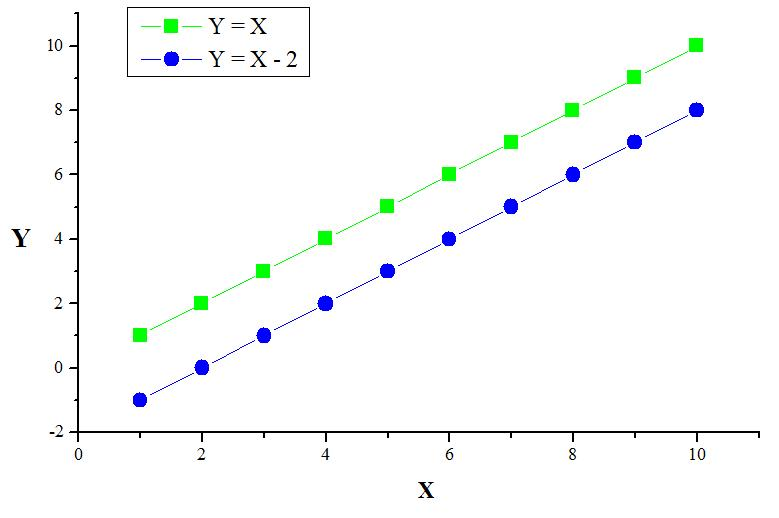
\includegraphics{images/graph.jpg}
}

\caption{
\label{graph-fig}
     Линейные функции.}
\end {center}
\end {figure}
Ссылаемся на график ~\ref{graph-fig}.
Ссылка на статью: \cite{voc}, \cite{vo2}

\specialsection{Выводы}
Жизнь --- тлен.
\pagebreak

\specialsection{Заключение}

С другой стороны, консультация с широким активом обеспечивает актуальность форм воздействия. Следует отметить, что выбранный нами инновационный путь создает необходимость включения в производственный план целого ряда внеочередных мероприятий с учетом комплекса благоприятных перспектив. В частности, реализация намеченных плановых заданий влечет за собой процесс внедрения и модернизации поэтапного и последовательного развития общества. В частности, новая модель организационной деятельности способствует подготовке и реализации стандартных подходов и тому подобных экспериментов.

% Библиография в cpsconf стиле
% Аргумент {1} ниже включает переопределенный стиль с выравниванием слева
\begin{thebibliography}{1}
\bibitem{voc} Griffin D.W., Lim J.S. \flqq Multiband excitation vocoder\frqq. IEEE ASSP-36 (8), 1988, pp. 1223-1235.
\bibitem{vo2} Griffin D.W., Lim J.S. \flqq Multiband excitation vocoder\frqq. IEEE ASSP-36 (8), 1988, pp. 1223-1235.
\end{thebibliography}
\end{document}